
\subsection{Results}

The tool-assisted Treatment group consistently outperformed the Control group across all six evaluative dimensions. These improvements ranged from medium to large effect sizes and remained statistically robust after controlling for non-normal data distributions and multiple hypothesis testing. Figure \ref{fig:distributions} shows the distributions of rating scores along each dimension of the evaluation rubric for both Control and Treatment groups. This section describes the exact statistical tests conducted on the evaluation dataset constructed in Section \ref{sec:scoring}, reporting their quantitative and qualitative results.

\subsubsection*{Statistical Approach}

We tested for normality using the Shapiro-Wilk test and found violations in at least one group for each dimension. For example, in the \textsc{Clarity} dimension, the Control group yielded $W = 0.8817$, $p = 0.0075$ (significant at $\alpha = 0.05$), indicating departure from normality. Similar violations occurred across other dimensions (e.g., \textsc{Relevance} in the Treatment group: $W = 0.8839$, $p = 0.0083$). Given these violations and the ordinal nature of Likert data, we used non-parametric Mann-Whitney U tests (one-tailed) for all group comparisons.
The rank-biserial correlation ($r$) was chosen as the most appropriate effect size for the Mann-Whitney U, where $r = 0.1$, $0.3$, and $0.5$ represent small, medium, and large effects, respectively.

\subsubsection*{Primary Findings}

All six dimensions showed statistically significant differences favoring the Treatment group. Median scores were higher in every case, with Mann-Whitney U tests indicating reliable group differences. Effect sizes were quantified using rank-biserial correlation ($r$), which represents the probability that a randomly selected Treatment participant scores higher than a randomly selected Control participant.
The results are summarized below:

\begin{description}
  \item [Clarity] Treatment (Median = 3.333) \textit{vs.} Control (Median = 3.000), $U = 439.5$, $p = .0063$. The rank-biserial correlation $r = 0.406$ indicates that 40.6\% of all possible pairwise comparisons between groups favor the Treatment group—a medium-to-large effect.

  \item [Relevance] Treatment (Median = 4.000) \textit{vs.} Control (Median = 3.000), $U = 496.5$, $p = .0001$, $r = 0.589$. This effect size means 58.9\% of pairwise comparisons favor Treatment—a large effect.

  \item [Persuasiveness] Treatment (Median = 3.333) \textit{vs.} Control (Median = 2.333), $U = 514.5$, $p < .0001$, $r = 0.646$. With 64.6\% of comparisons favoring Treatment, this represents a large effect.

  \item [Concern for Long-Term Consequences] Treatment (Median = 4.000) \textit{vs.} Control (Median = 3.000), $U = 548.5$, $p < .0001$, $r = 0.755$. The strongest effect observed, with 75.5\% of pairwise comparisons favoring Treatment.

  \item [Practical Usefulness] Treatment (Median = 3.667) \textit{vs.} Control (Median = 2.000), $U = 531.5$, $p < .0001$, $r = 0.701$. Another large effect, with 70.1\% of comparisons favoring Treatment.

  \item [Awareness of Context] Treatment (Median = 4.000) \textit{vs.} Control (Median = 2.667), $U = 551.0$, $p < .0001$, $r = 0.763$. The second-strongest effect, with 76.3\% of comparisons favoring Treatment.
\end{description}

\subsubsection*{Process Measures}

Self-assessment data provided supporting evidence for the treatment mechanisms. Despite investing 35\% more time in the task (Treatment: M = 16:12 \textit{vs.} Control: M = 12:00), Treatment participants reported higher confidence in their responses (M = 4.52 \textit{vs.} M = 4.36). Treatment participants also rated the tool-generated summaries positively for supporting reflection (M = 4.32/5) and perceived real-world utility (M = 4.44/5), suggesting genuine value beyond novelty effects.

\subsubsection*{Robustness Checks}

To validate the reliability of these findings, we conducted the following robustness checks:

\begin{description}
  \item[Confidence Intervals] Non-parametric 95\% bootstrap confidence intervals were computed for median differences. All intervals excluded zero, confirming statistical significance. Representative examples include \textsc{Clarity} $[0.000, 1.333]$, \textsc{Persuasiveness} $[0.333, 2.000]$, and \textsc{Awareness} $[1.000, 2.000]$.

  \item[Multiple Comparisons] Both Bonferroni correction (adjusted $\alpha = 0.0083$) and False Discovery Rate (FDR) correction were applied to control for inflated Type I error rates across six simultaneous tests. All comparisons remained statistically significant under both correction methods.
\end{description}

\subsubsection*{Summary}

Across every dimension, the Treatment group showed statistically and practically significant improvements over the Control group. These findings were consistent across multiple analytical lenses—median comparisons, effect sizes, time data, self-report metrics, and error-correction methods—providing robust evidence for the tool's effectiveness in enhancing ethical decision-making quality.

\begin{figure*}[t]
  \centering
  % First row
  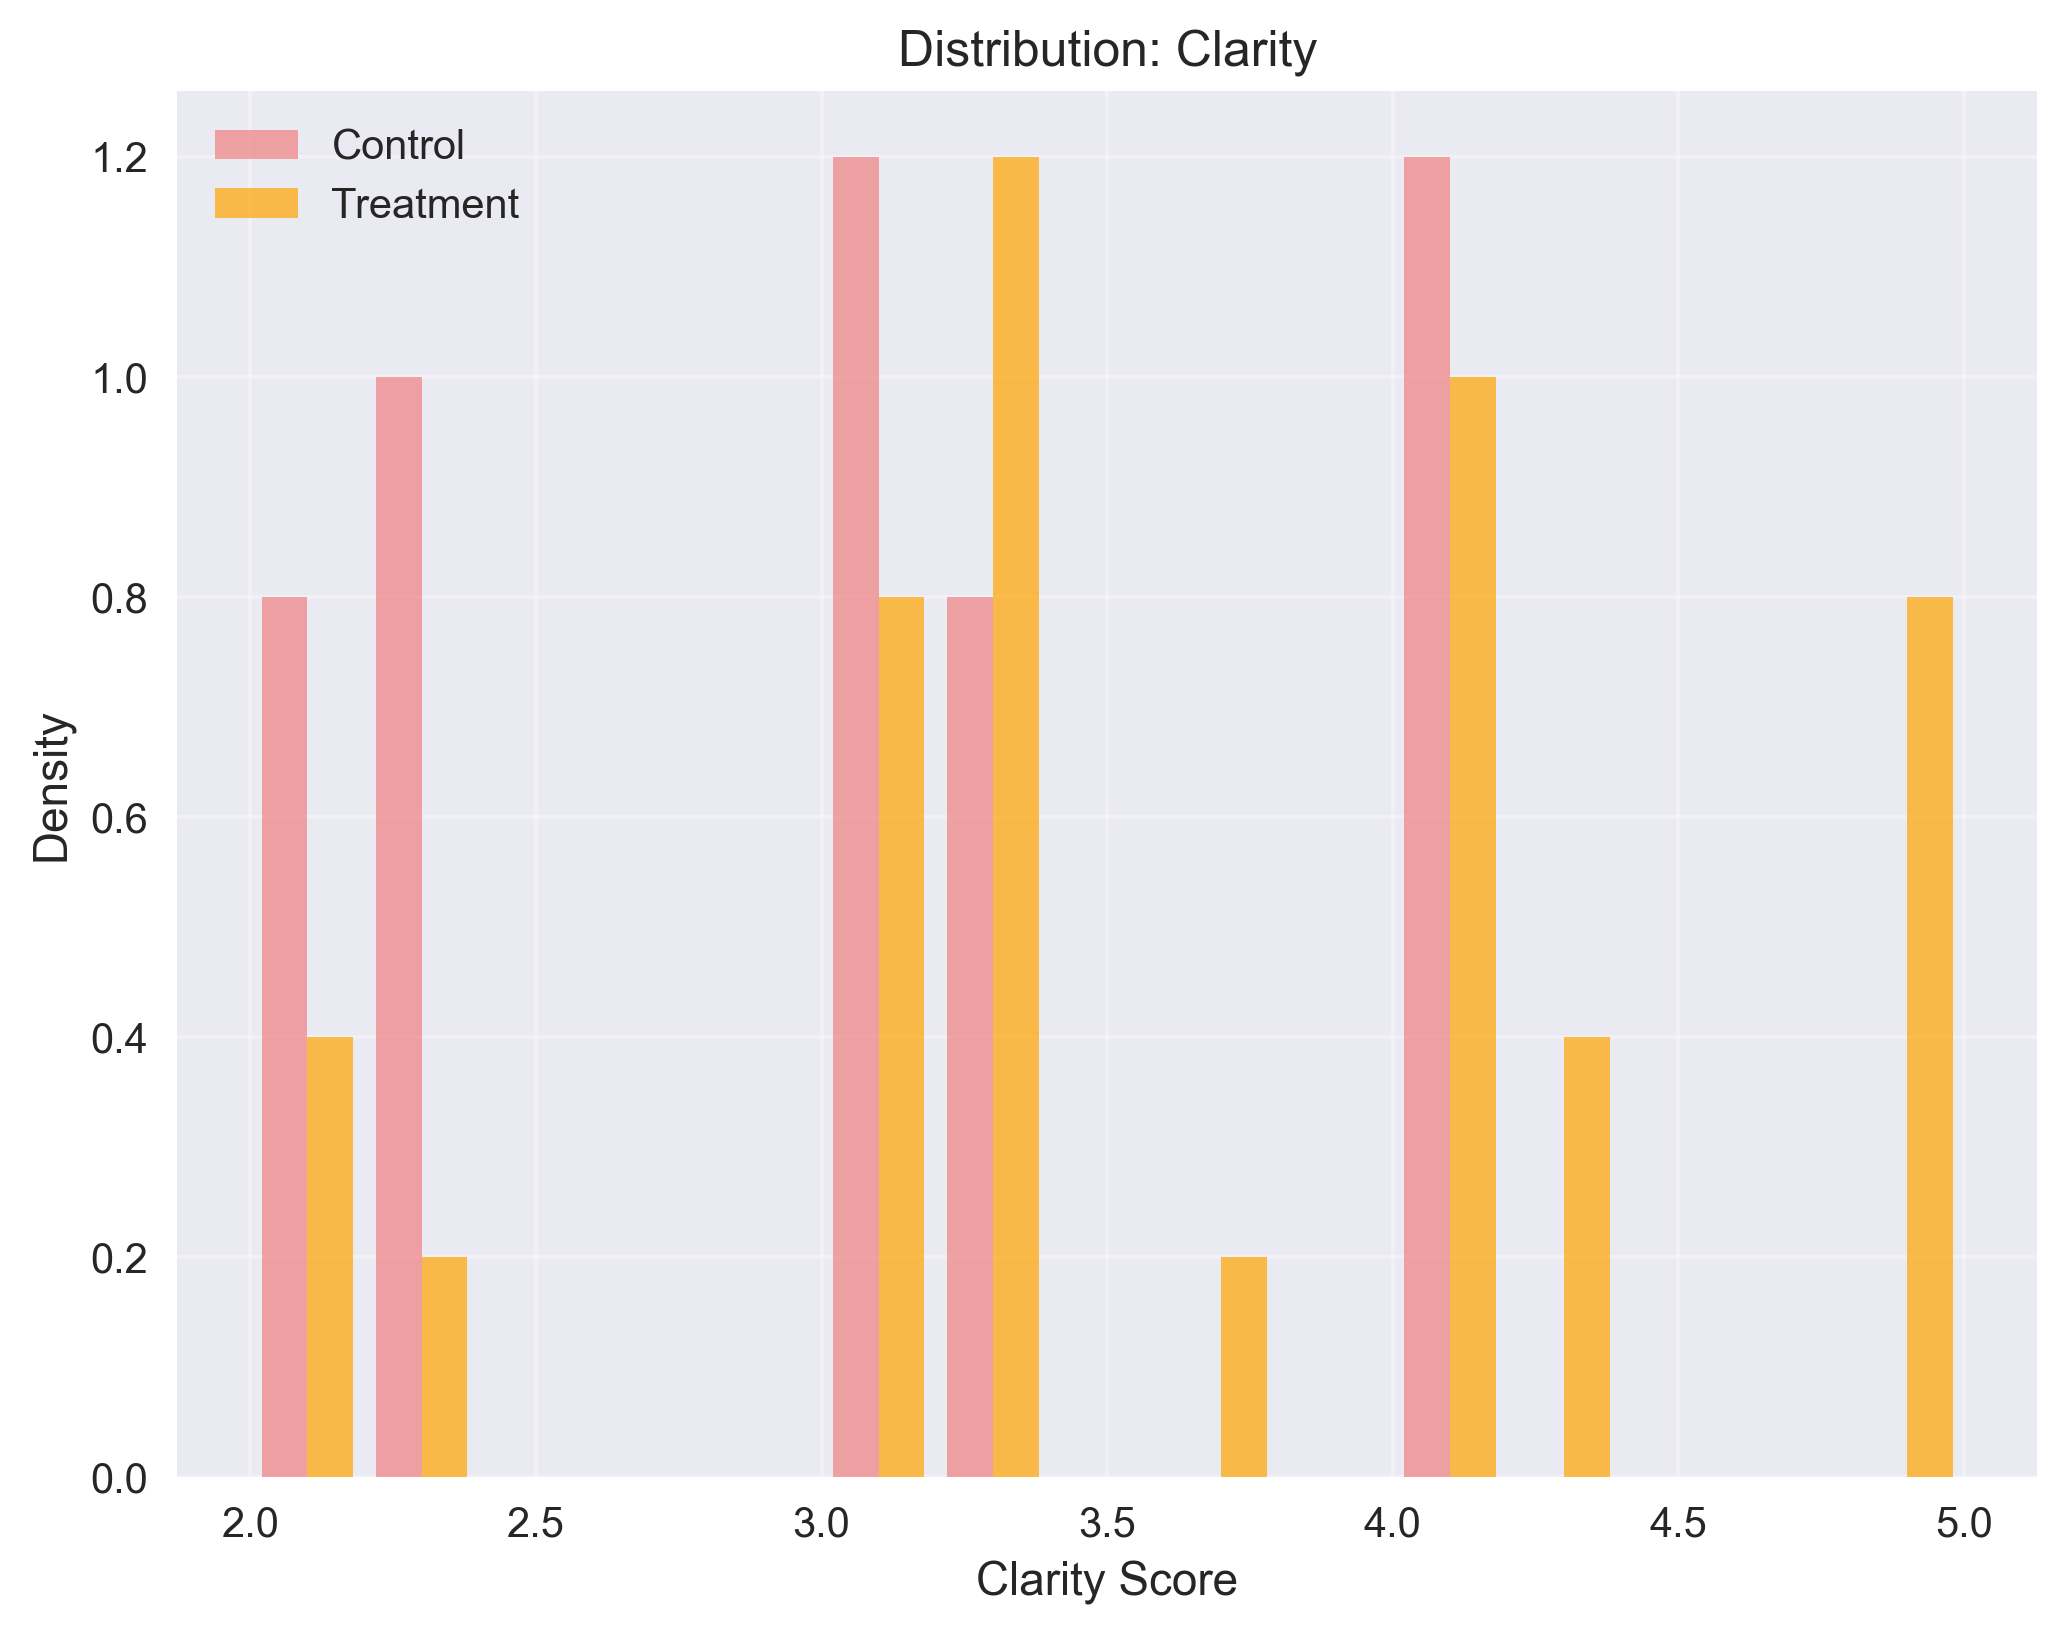
\includegraphics[width=0.3\textwidth]{plots/distribution_clarity.png} \hfill
  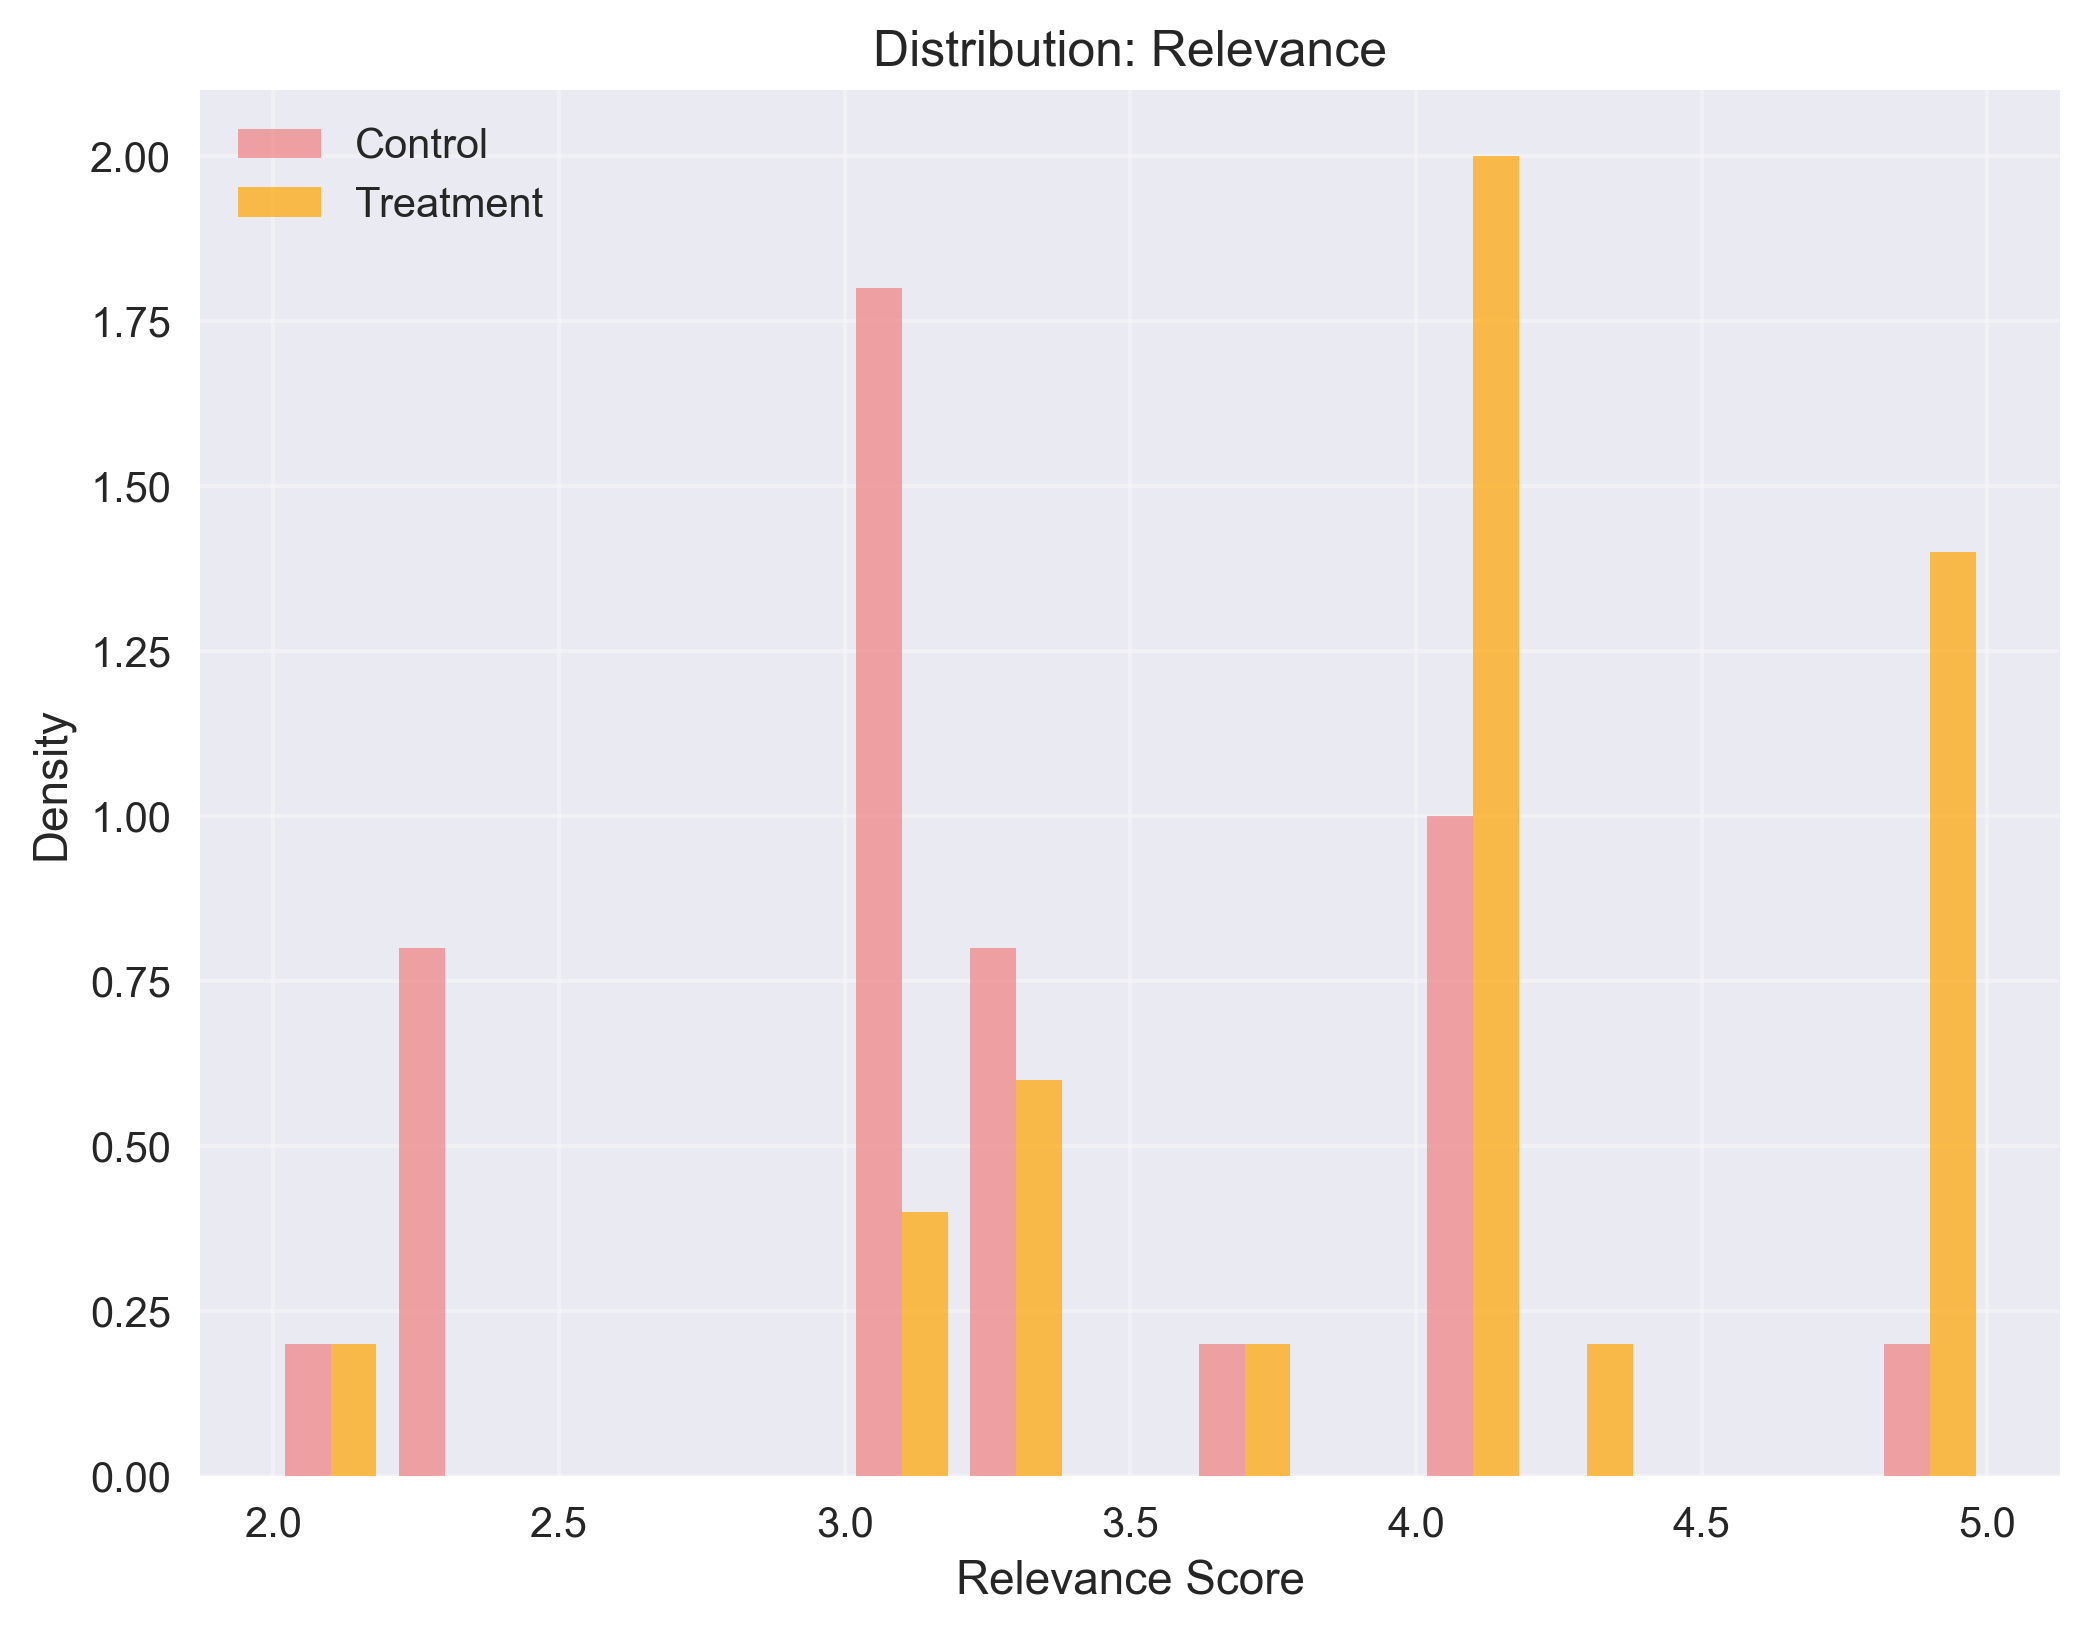
\includegraphics[width=0.3\textwidth]{plots/distribution_relevance.png} \hfill
  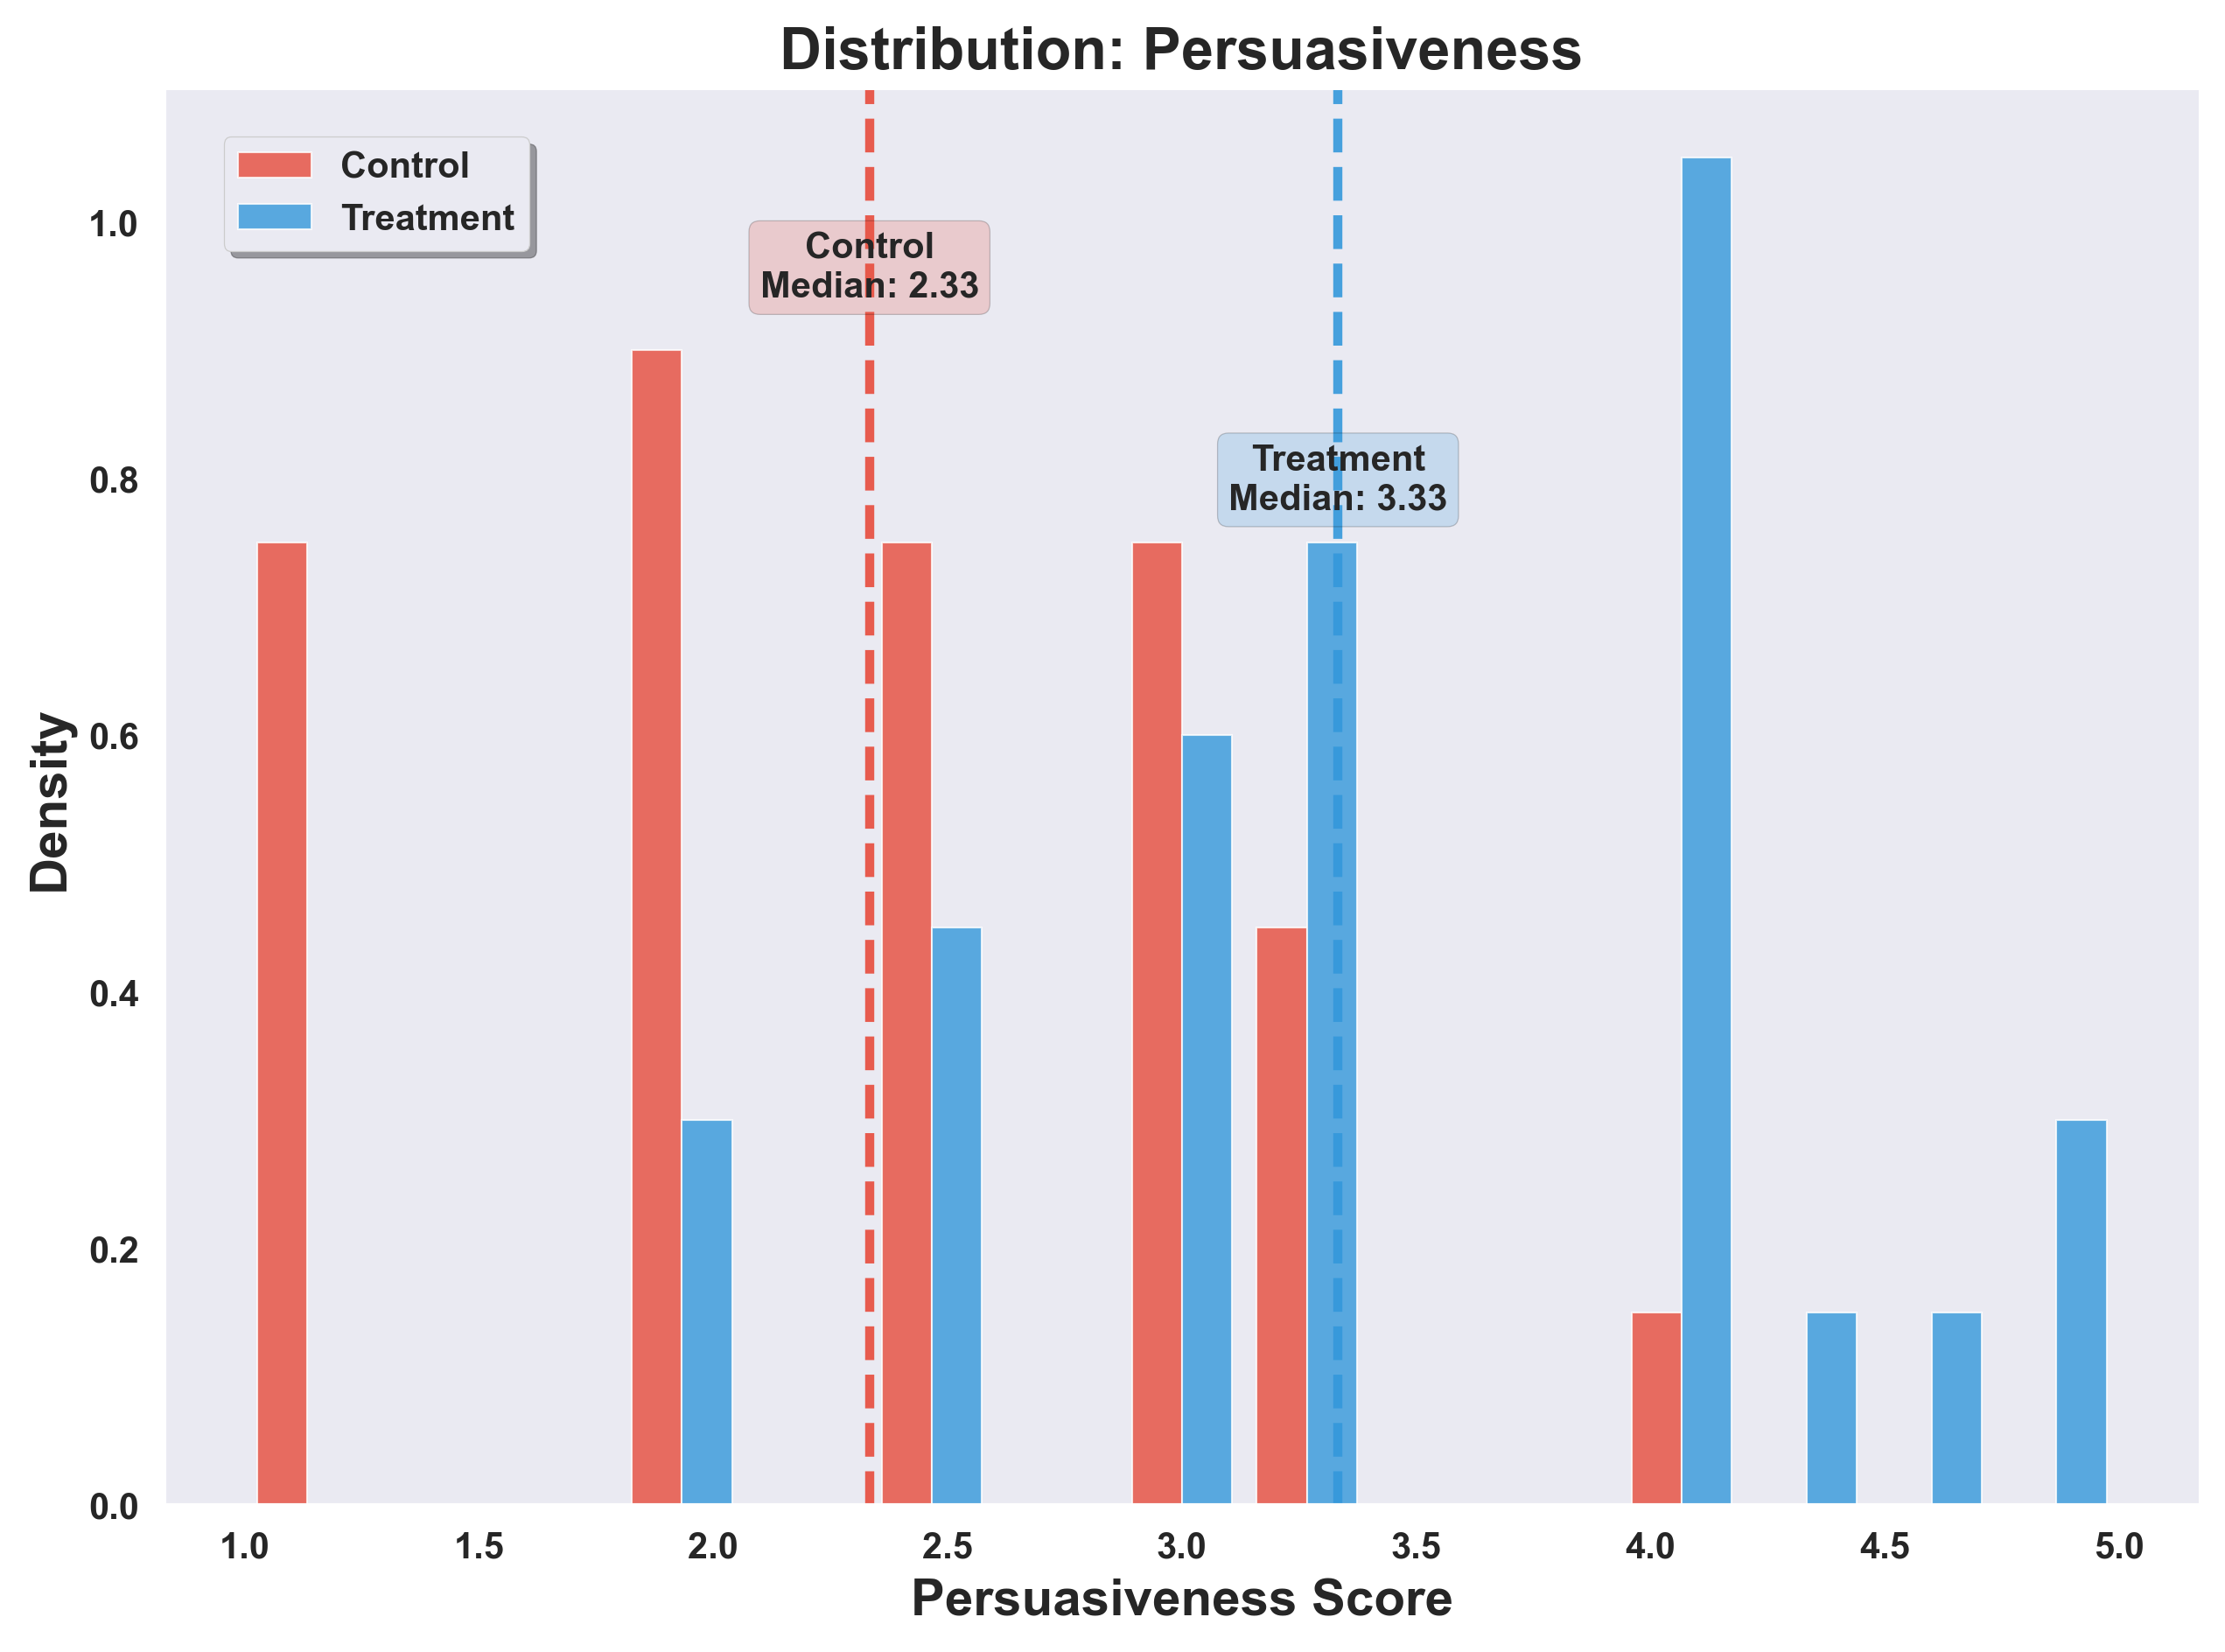
\includegraphics[width=0.3\textwidth]{plots/distribution_persuasiveness.png}

  \vspace{1em} % vertical spacing between rows

  % Second row
  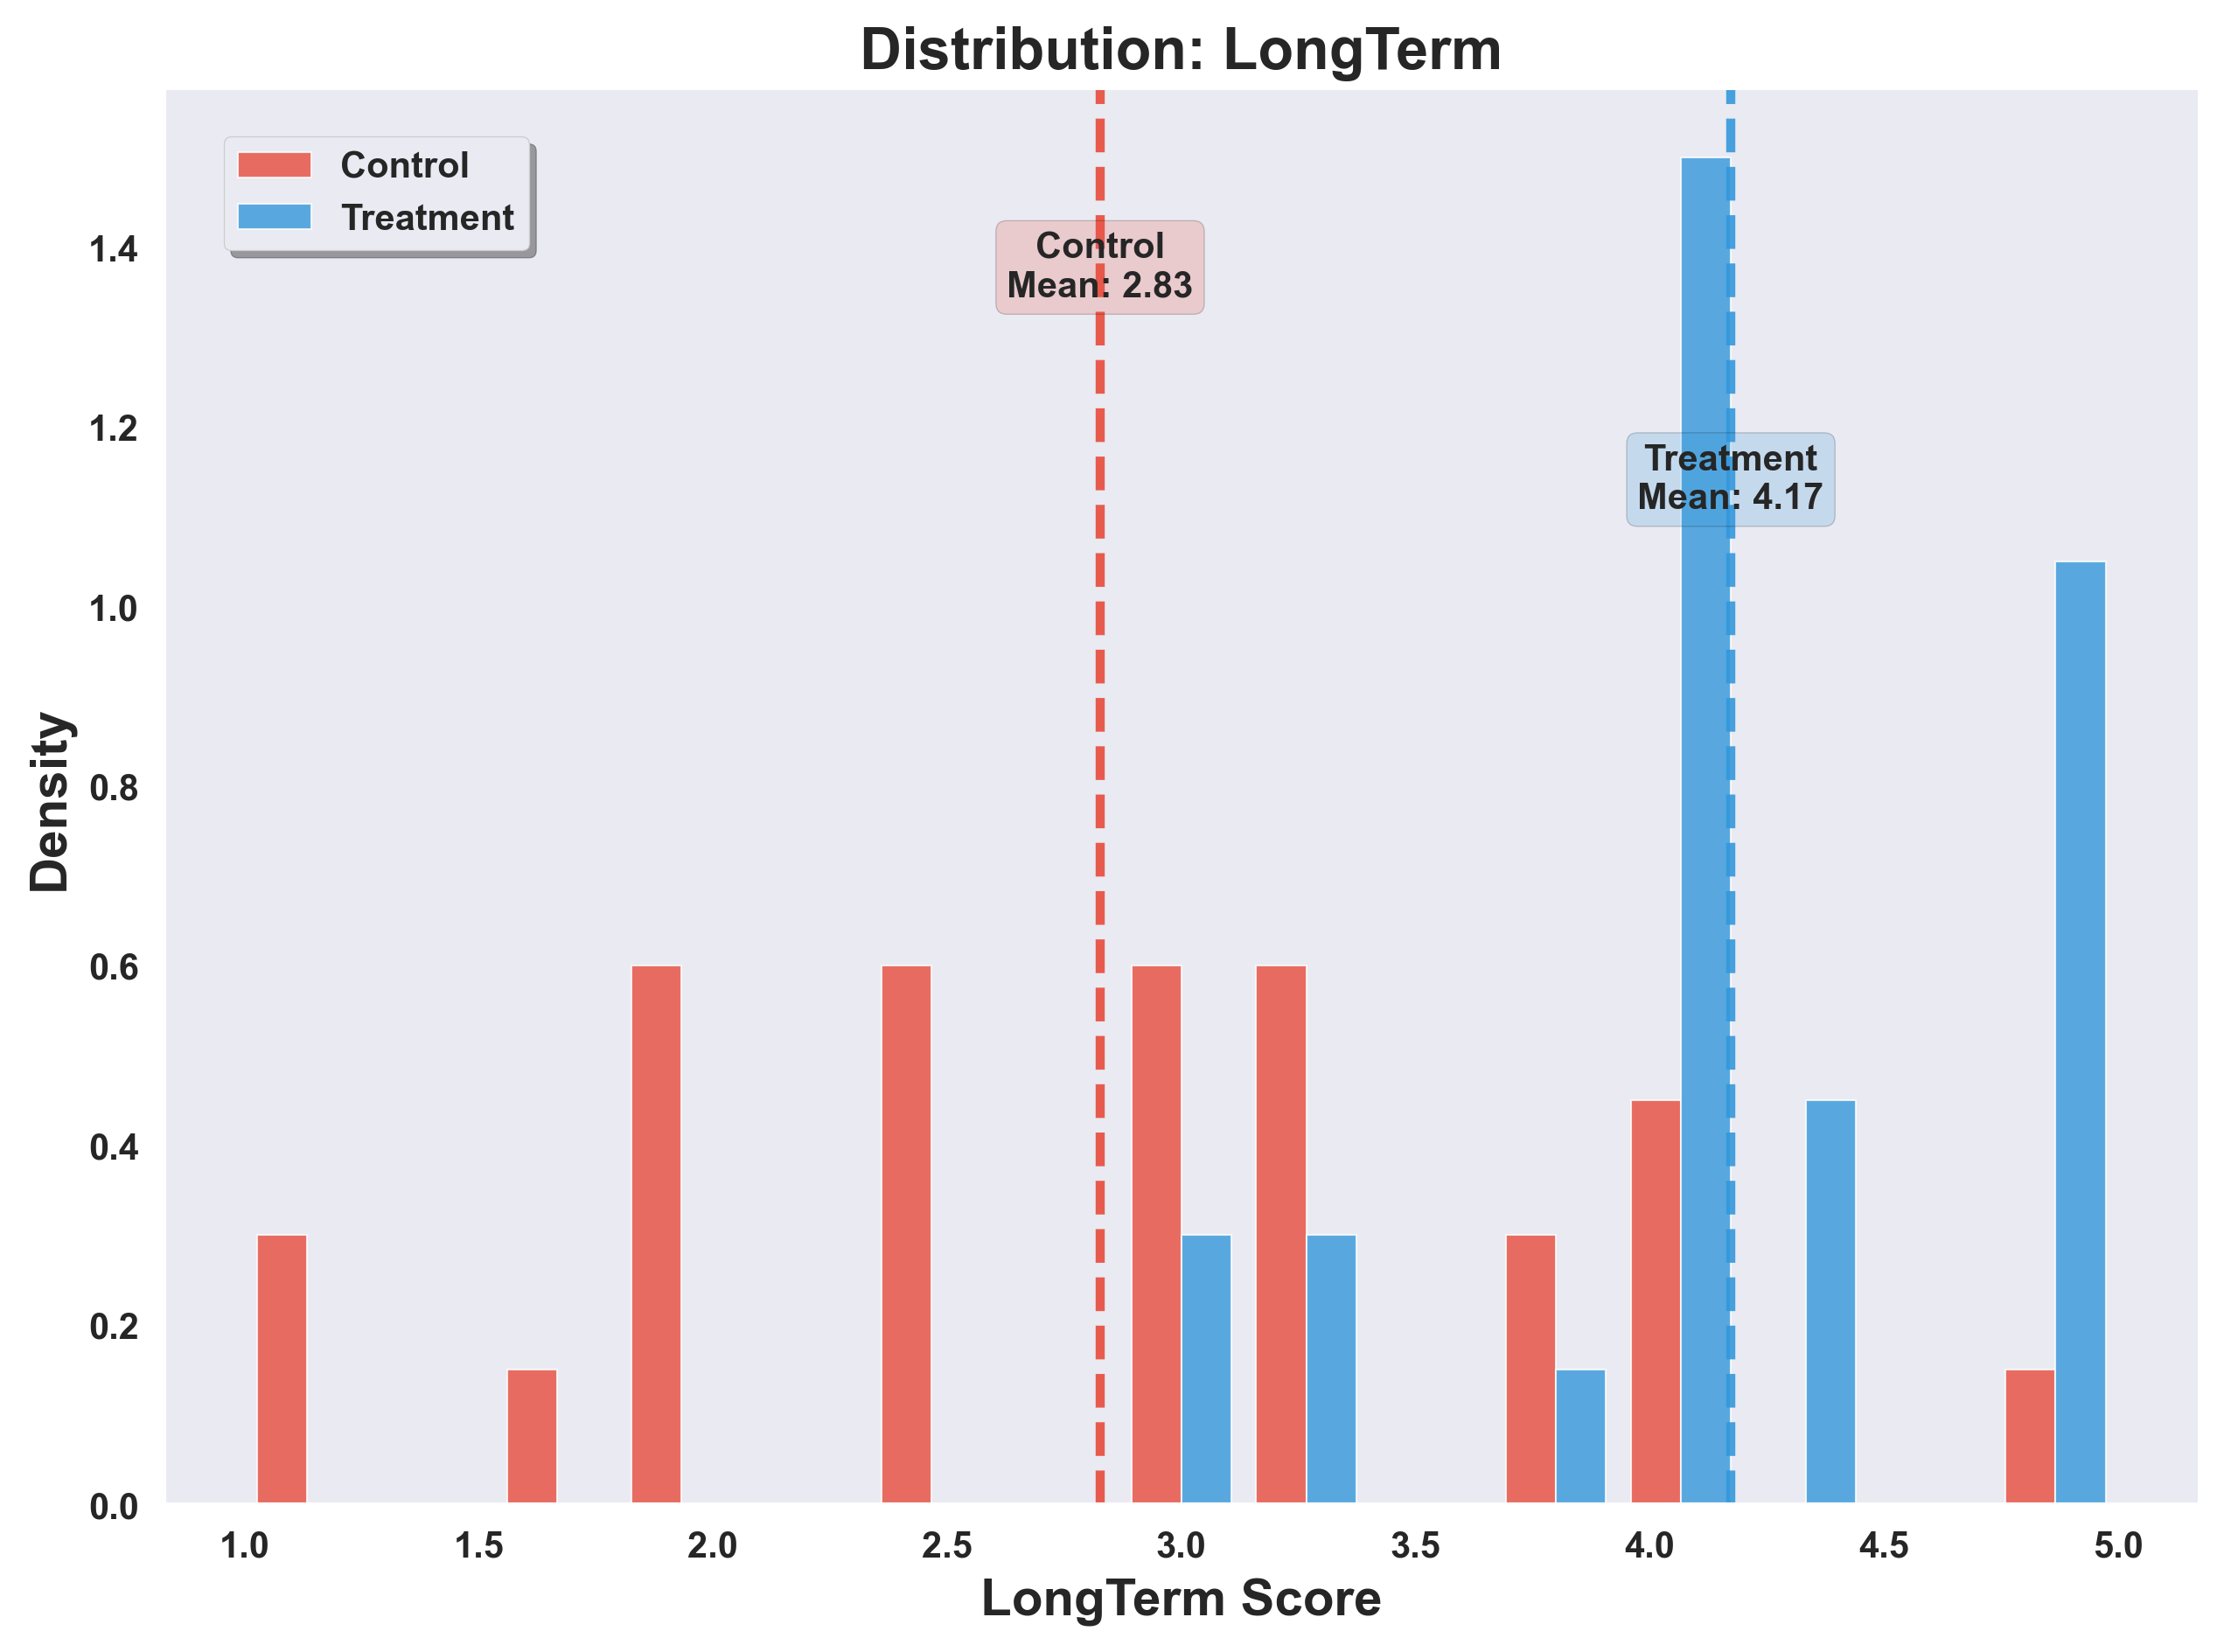
\includegraphics[width=0.3\textwidth]{plots/distribution_longterm.png} \hfill
  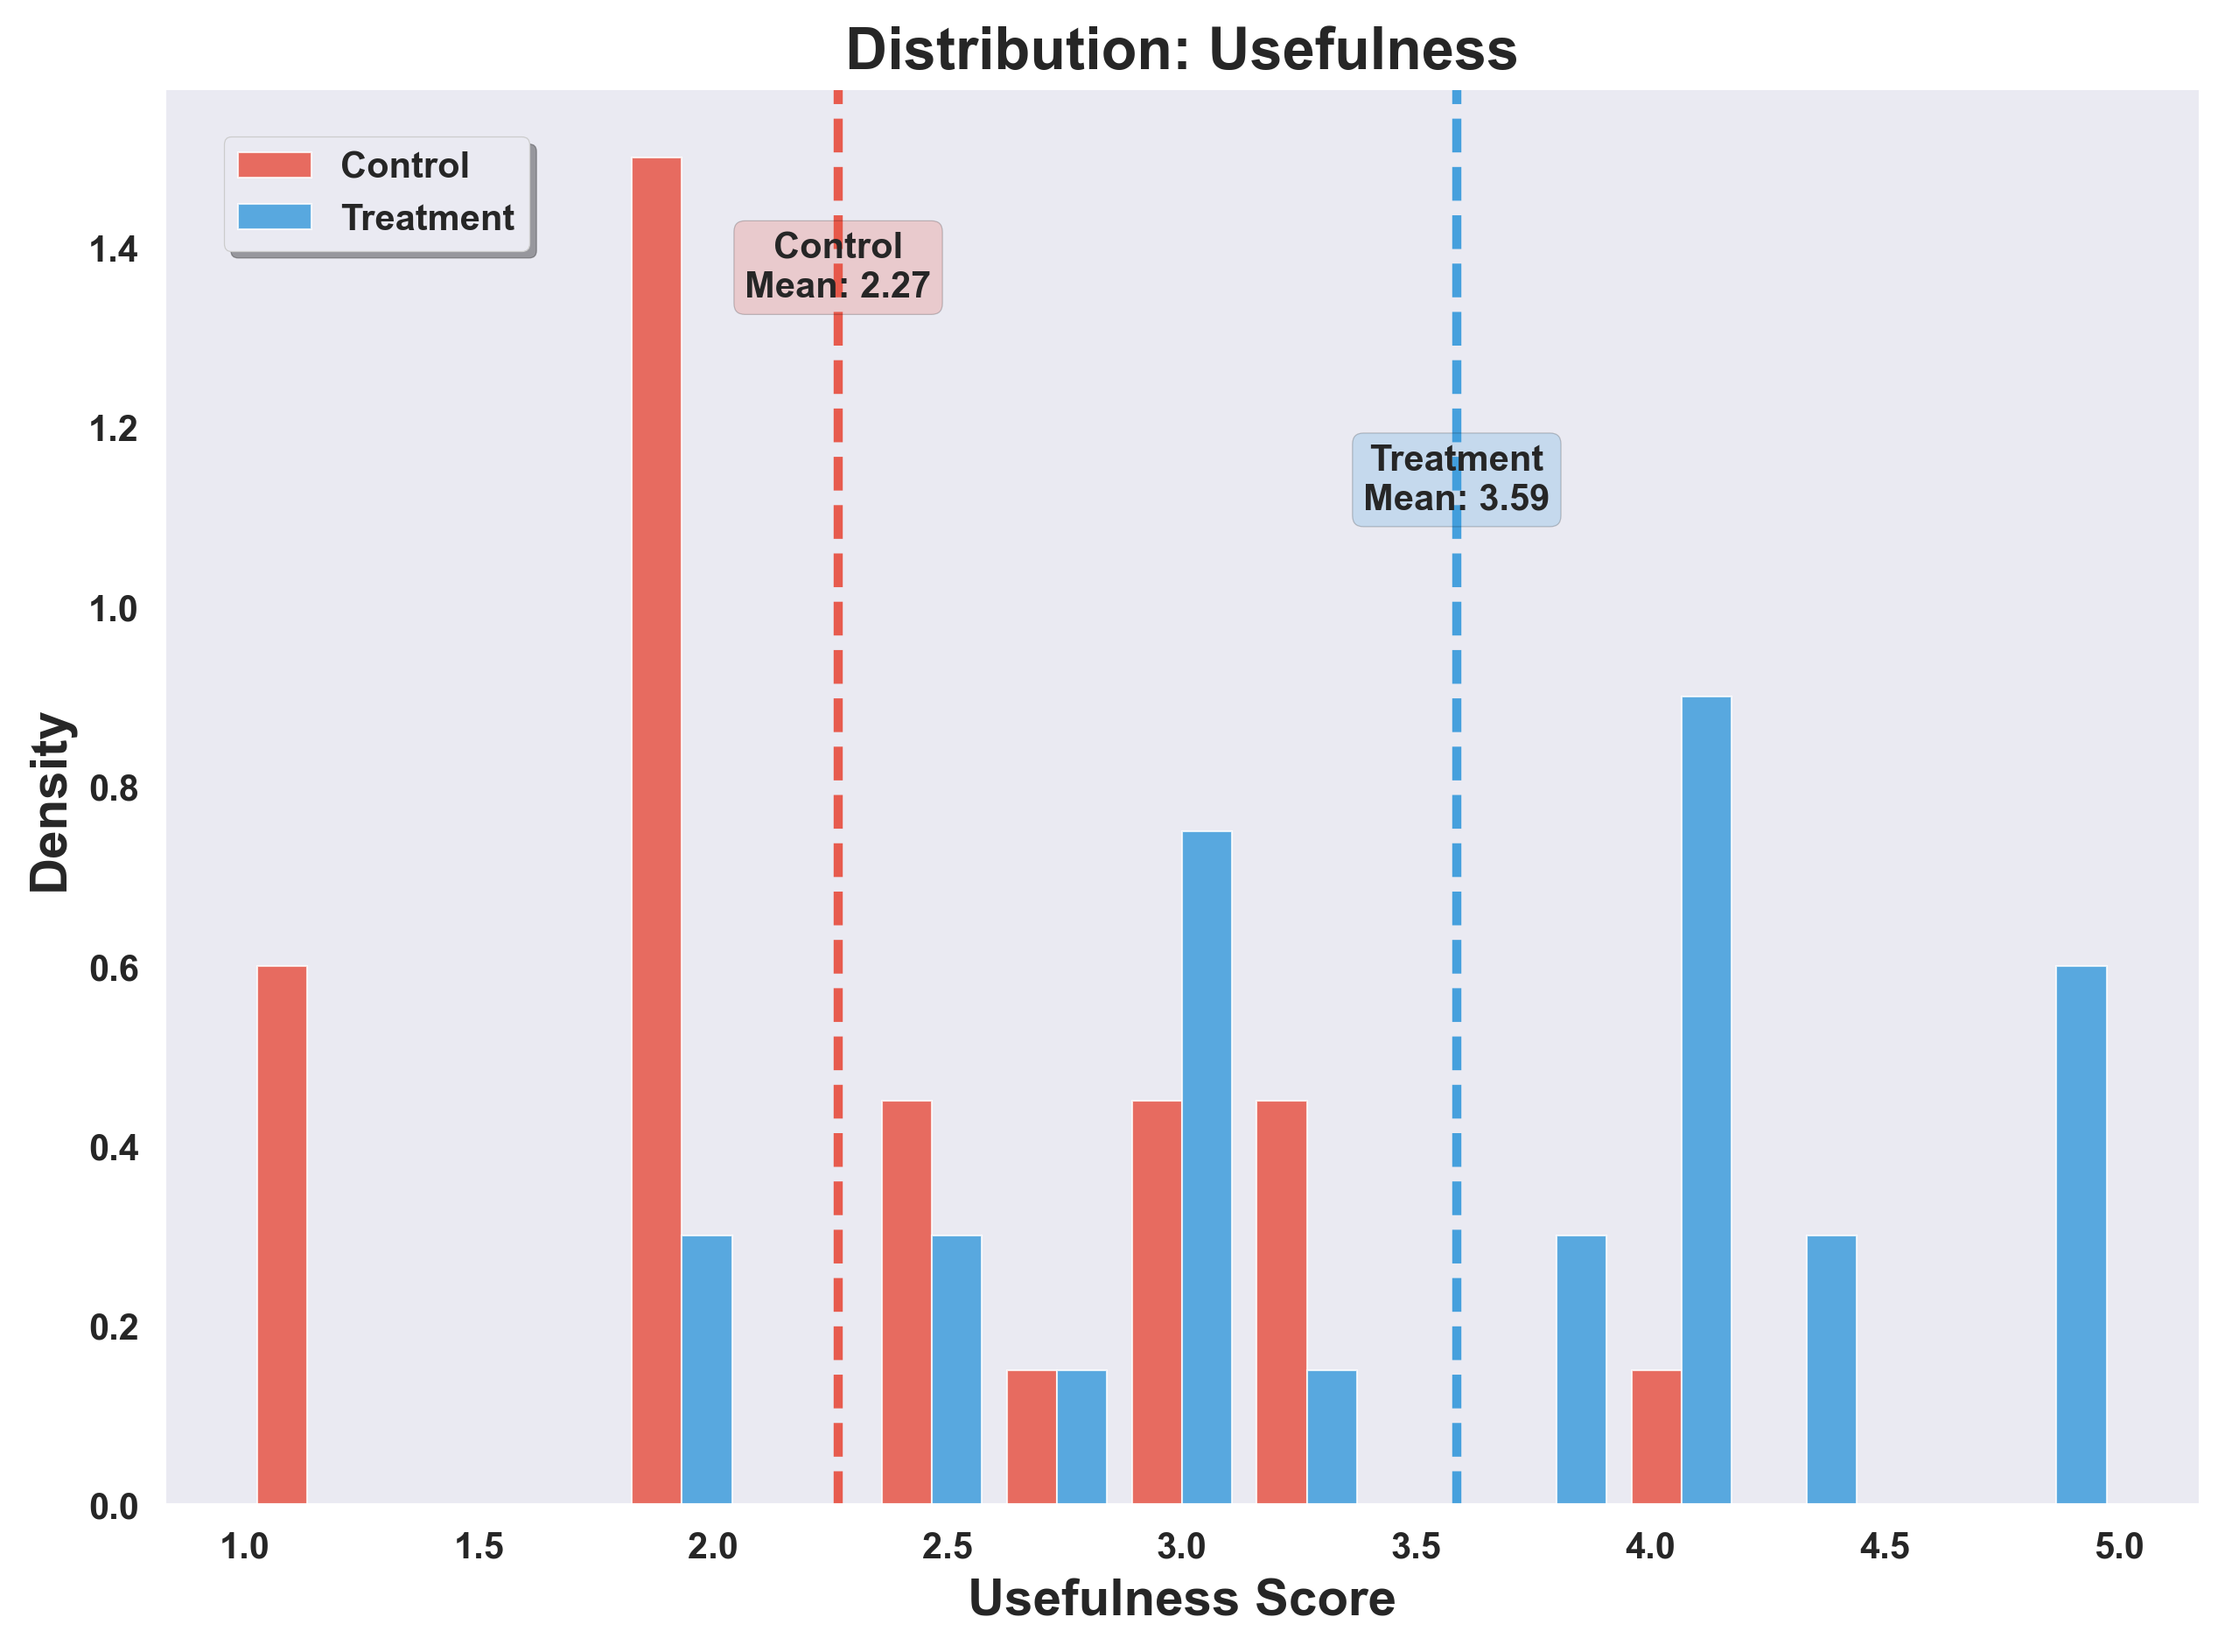
\includegraphics[width=0.3\textwidth]{plots/distribution_usefulness.png} \hfill
  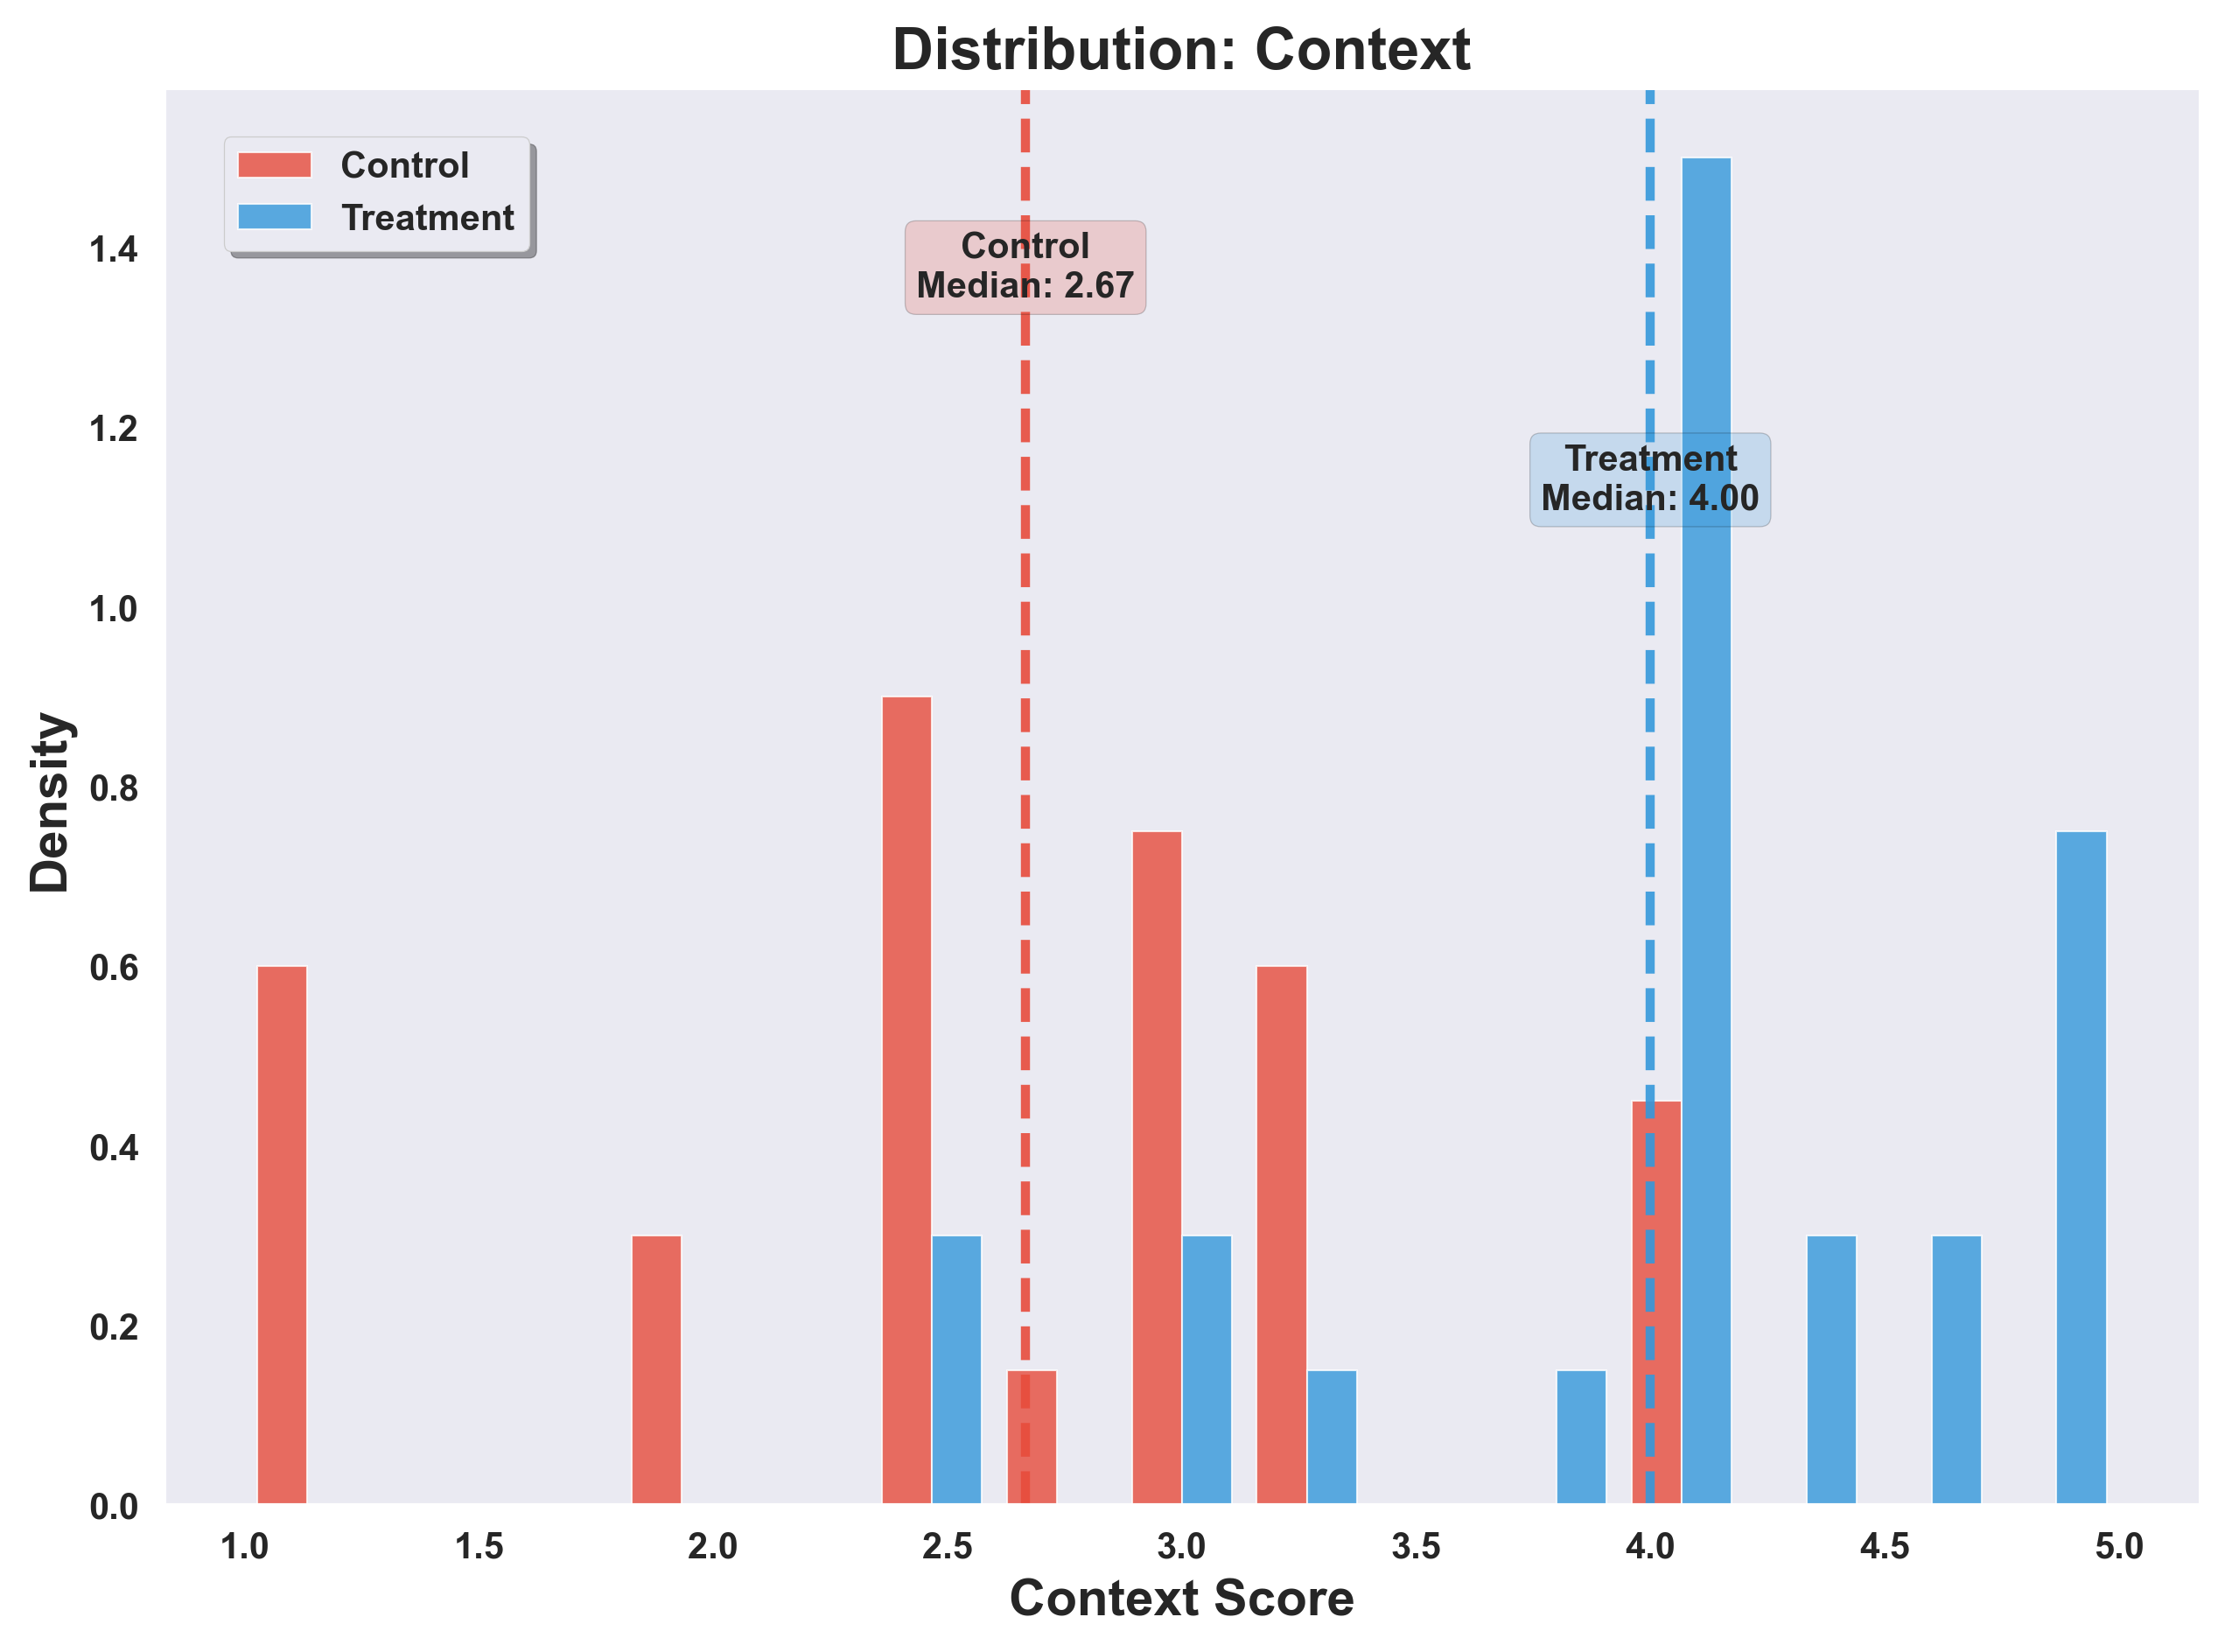
\includegraphics[width=0.3\textwidth]{plots/distribution_context.png}

  \caption{
    Score distributions for each rubric dimension across groups.
    Density plots compare Control (red) and Treatment (blue) groups across all six evaluation dimensions: (top row, left to right) Clarity, Relevance, Persuasiveness: (bottom row, left to right) Concern for Long-Term Consequences, Practical Usefulness, and Awareness of Context. Vertical dashed lines indicate group means. In all dimensions, the Treatment group demonstrates a rightward shift, reflecting higher average scores and greater distributional density in the upper range.
  }
  \label{fig:distributions}
\end{figure*}
